\section{System and Raspberry Pi specifications}
\section{Objective 1: \texttt{mpbenchmark}}
\section{Objective 2: \texttt{MobileNet}}
\section{Objective 3: \texttt{DeBaTE-FI} platform}

\begin{lstlisting}[
	caption={Command line arguments of the new \texttt{mpbenchmark} solution.},
	label={lst:main_file_cpp}
	]
	int main(int argc, char *argv[]){
		int engine{};
		int numThreads{};
		
		if (argc > 1) {
			engine = std::atoi(argv[1]); // Convert the argument to an integer
		}
		
		if (argc > 2) {
			numThreads = std::atoi(argv[2]); // Convert the argument to an integer
		}
		
		// If the number of threads is not specified, default to the maximum available
		if (numThreads == 0) {
			numThreads = std::thread::hardware_concurrency();
		}	
		// ignore the other remaining code...
	}
\end{lstlisting}


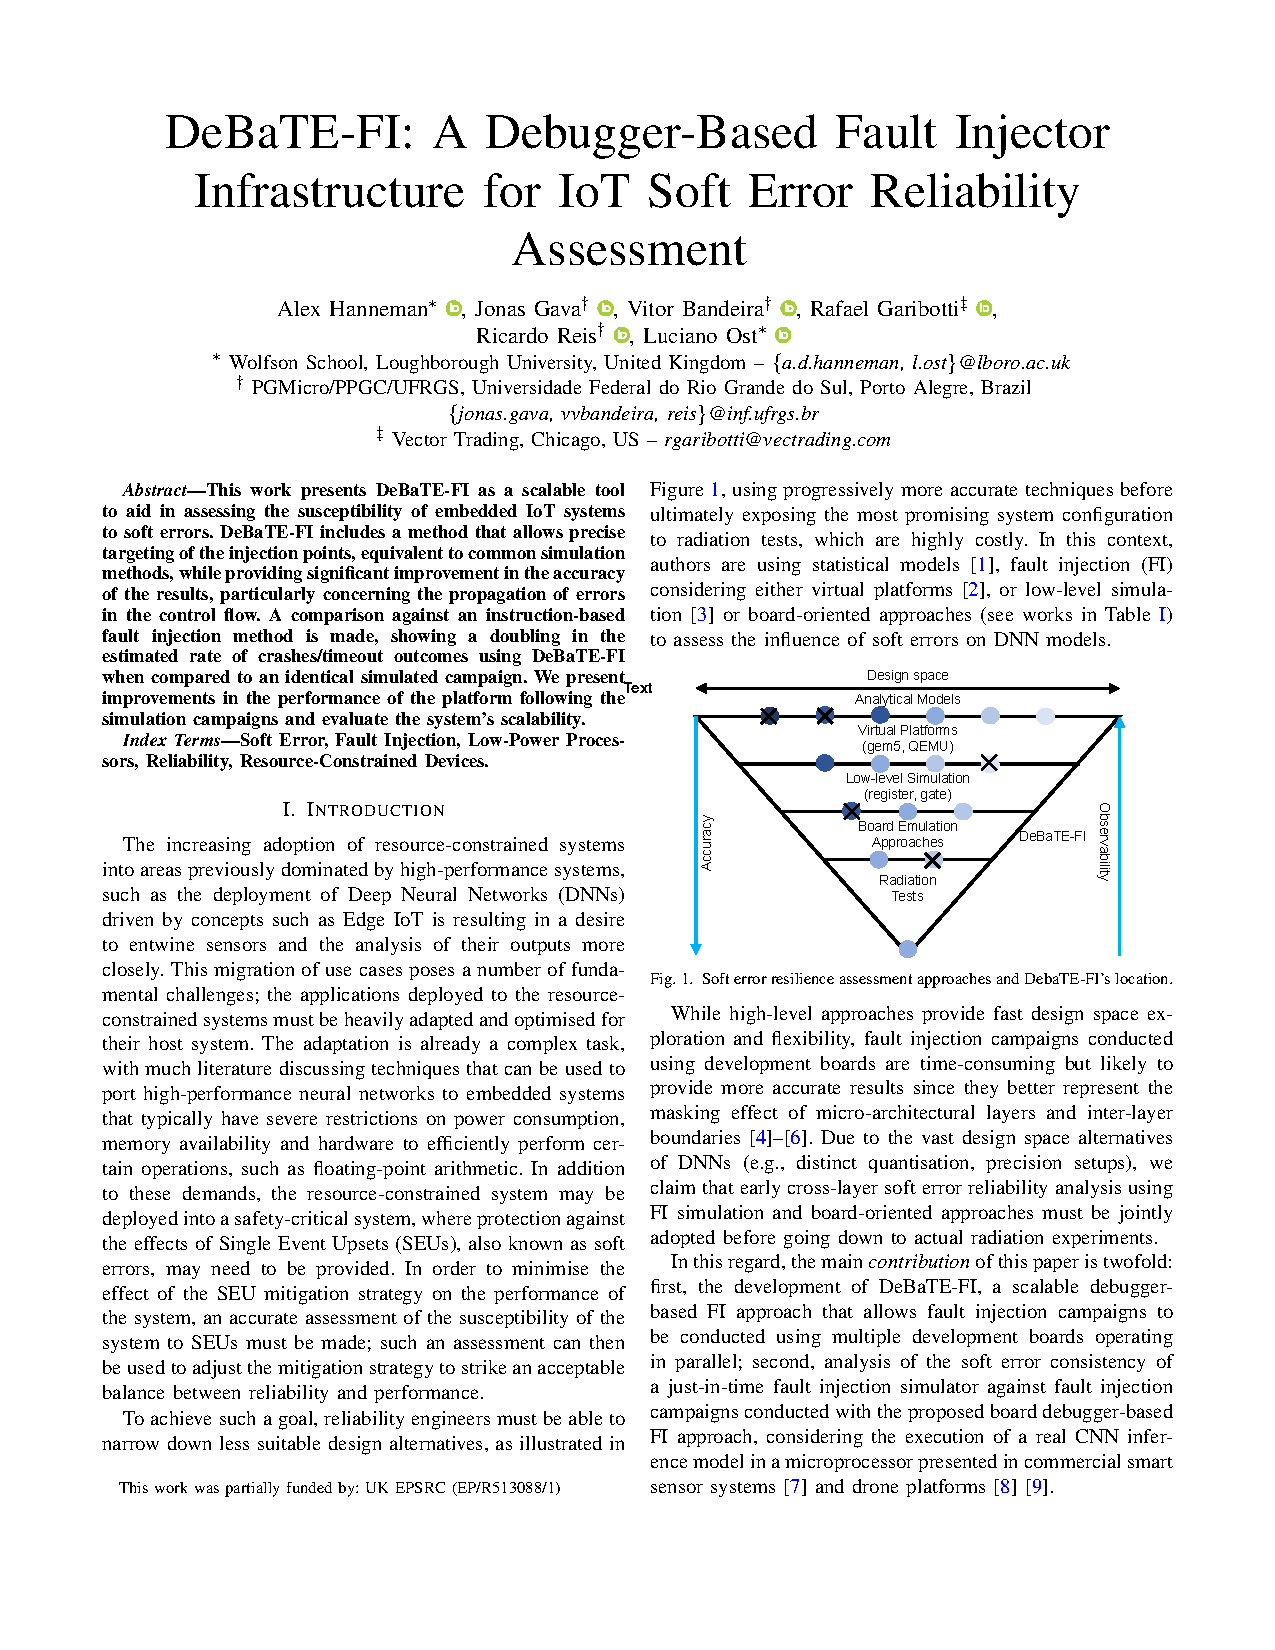
\includepdf[
pages=-,
addtotoc={1, section, 1, DeBaTE-FI platform publication(maybe remove?), appendix:debate_fi},
pagecommand={\label{appendix:debate_fi}}
]{~/Documents/Part_D_Modules/Individual_Project/Individual_report/files/Debate_FI_platform.pdf}


